\chapter{Fonctions de phase}

\section{Présentation}

Une BSDF (Bidirectional Scattering Distribution Function) permet de décrire et simuler la façon dont la lumière est dispersée par une surface. Une \textbf{fonction de phase} $\rho (\omega_{i}\longrightarrow\omega_{o})$ est son analogue volumétrique. Elle permet de décrire la façon dont la lumière se disperse \textit{à l'intérieur} du volume. On peut la lire comme une pdf donnant la probabilité qu'un photon arrivant sur une particule dans la direction $\omega_{i}$ en ressorte par la direction $\omega_{o}$. De ce fait, une fonction de phase possède une contrainte de normalisation :
\large \begin{equation}\label{eq:condition_de_normalisation}
    \int_{\Omega4\pi}\rho(\omega_{i}\longrightarrow\omega_{o})d\omega' = 1
.\end{equation} \normalsize \newline\par

Dans beaucoup de milieux participants, la fonction de phase est \textbf{isotropique}. Celle-ci ne dépend que de l'\textit{angle de phase} $\theta$ entre le rayon incident $\omega_{i}$ et le rayon sortant $\omega_{o}$. On se contente alors d'écrire $\rho(cos\theta)$. La dispersion est identique dans toutes les directions pour un angle donné.\par
Il est également intéressant de noter que les fonctions de phases sont des fonctions réciproques, les deux directions incidentes et sortantes peuvent être interchangées et la valeur de la fonction de phase restera la même :
\large \begin{equation}\label{eq:fp_reciprocité}
    \rho(\omega_{i}\longrightarrow\omega_{o}) = \rho(\omega_{o}\longrightarrow\omega_{i})
.\end{equation} \normalsize \newline\par


Tout comme les BSDF, il existe de nombreux modèles de fonctions de phase qui produisent des effets différents. Certains peuvent facilement être décrits avec un seul paramètre, mais d'autres plus complexes demandent une équation bien plus grosse et difficilement utilisables dans un algorithme. Il est donc parfois plus simple de diviser une fonction de phase $\rho(\omega_{i}\longrightarrow\omega_{o})$ complexe en plusieurs fonctions de phases $\rho_{k}(\omega_{i}\longrightarrow\omega_{o})$ plus simples. Nous avons l'égalité suivante :
\large \begin{equation}\label{eq:fp_somme}
    \rho(\omega_{i}\longrightarrow\omega_{o}) = \sum\limits_{k=1}^n w_{k}\rho_{k}(\omega_{i}\longrightarrow\omega_{o})
,\end{equation} \normalsize
où chacune des fonctions $\rho_{k}$ possède un poids $w_{k}$ dans l'équation, avec la somme de tous les $w_{k}$ qui égale 1 afin de maintenir la \textit{condition de normalisation} (formule \ref{eq:condition_de_normalisation}).


\section{Henyey-Greenstein}
\label{explication_parametre_g}

Henyey et Greenstein (1941) ont introduit une fonction de phase qui est aujourd'hui beaucoup utilisée car elle ne dépend que d'un paramètre $-1 \leq g \leq 1$ et décrit les effets de \textit{backscattering} tout comme ceux de \textit{forwardscattering} :
\large
$$\rho_{HG}(cos\theta) = \frac{1}{4\pi} \frac{1-g^2}{(1+g^2-2g(cos\theta))^{3/2}}.$$
\normalsize
Le paramètre $g$ n'est pas arbitraire et peut être calculé avec la formule suivante :
\large
$$g = \int_{\Omega4\pi}\rho(\omega_{i}\longrightarrow\omega_{o})(\omega_{i}\cdot\omega_{o})d\omega_{o} = 2\pi\int_{0}^{\pi}\rho(cos\theta)cos\theta sin\theta d\theta.$$
\normalsize
\par
La valeur de $g$ induit certains effets de dispersion dans la fonction de phase $\rho_{HG}$. Si $g<0$ alors la fonction de phase décrit principalement des effets de \textit{backscattering} (Figure \ref{fig:backscattering}). Si $g>0$, on a à l'inverse principalement du \textit{forwardscattering} (Figure \ref{fig:forwardscattering}). Enfin, comme on s'y attend, si $g=0$, la fonction de phase est isotropique.\newline\par

\begin{figure}
   \begin{minipage}[c]{.46\linewidth}
      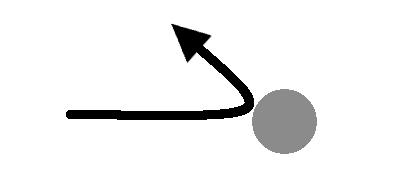
\includegraphics[width=80mm]{backscattering.png}
      \caption{Backscattering, $g<0$}
      \label{fig:backscattering}
   \end{minipage} \hfill
   \begin{minipage}[c]{.46\linewidth}
      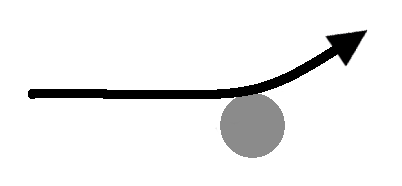
\includegraphics[width=80mm]{forwardscattering.png}
      \caption{Forwardscattering, $g>0$}
      \label{fig:forwardscattering}
   \end{minipage}
\end{figure}

\section{Schlick}

La fonction de phase de Henyey et Greenstein est cependant lourde à calculer à cause de la puissance présente au dénominateur. Blasi, Le Saëc et Schlick (1993) ont développé une approximation de $\rho_{HG}$ qui évite cette puissance et qui est donc plus utilisée en informatique graphique, où la forme exacte de la fonction de phase de Henyey et Greenstein n'est pas nécessaire.
\large
$$\rho_{Schlick}(cos\theta) = \frac{1}{4\pi} \frac{1-k^2}{(1-kcos\theta)^2},$$
\normalsize
où le paramètre $k$ joue le même rôle que le terme $g$ : $k=-1$  un backscattering total, $k=0$ implique l'isotropie du milieu, $k=1$ correspond à un forwardscattering total. Pharr et Humphreys (2004) ont trouvé que définir $k$ comme :
\large
$$k = 1,55g-0,55g^2,$$
\normalsize
était une bonne façon d'avoir une relation directe entre $k$ et $g$ avec laquelle $\rho_{Schlick}$ avoisine très bien $\rho_{HG}$.

\section{Rayleigh}

Le modèle de Rayleigh décrit une dispersion de la lumière dans un milieu composé de petites particules, jusqu'à un dixième de la longueur d'onde de la lumière.
\large
$$\rho_{R}(cos\theta) = \frac{3}{16\pi}(1+cos^2\theta).$$
\normalsize
Ce modèle permet par exemple de simuler la diffusion de la lumière dans le ciel. En le suivant, on retrouve ainsi sa couleur bleue.


\section{Mie}

La théorie de Rayleigh ne fonctionne que pour des particules de petites tailles. Lorsque celles-ci dépassent le dixième de leur longueur d'onde (aérosols, poussière, goutellettes d'eau), il faudrait passer à la théorie de Mie. Cela dit, son application est compliquée. La figure \ref{fig:cloud_pf} présente une fonction de phase pour un nuage, trouvée avec la théorie de Mie.

\begin{figure}[h!]
\centering
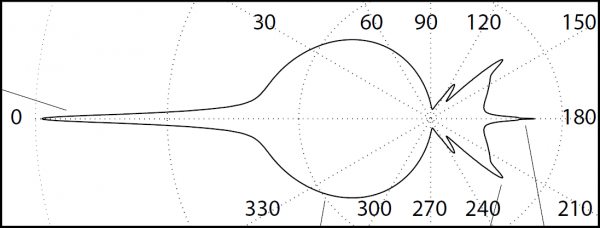
\includegraphics[width=150mm]{cloud_phase_function.png}
\caption{Fonction de phase d'un nuage}
\label{fig:cloud_pf}
\end{figure}

Aussi, plutôt que d'utiliser cette fonction de phase compliquée, on choisit généralement une composition de plusieurs fonctions de phase de Henyey et Greenstein (ou Schlick). C'est ici, par exemple, qu'est utilisée la formule \ref{eq:fp_somme} :
\large
$$\rho(\omega_{i}\longrightarrow\omega_{o}) = \sum\limits_{k=1}^n w_{k}\rho_{k}(\omega_{i}\longrightarrow\omega_{o}).$$
\normalsize